\documentclass[12pt,a4paper]{article}

% Encoding and fonts
\usepackage[utf8]{inputenc}
\usepackage[T1]{fontenc}
\usepackage{lmodern}

% Mathematics
\usepackage{amsmath}
\usepackage{amssymb}
\usepackage{amsfonts}
\usepackage{amsthm}
\usepackage{mathtools}

% Layout
\usepackage[margin=1in]{geometry}
\usepackage{setspace}
\doublespacing

% References and links
\usepackage[hidelinks]{hyperref}

% Figures
\usepackage{graphicx}
\graphicspath{{figures/}}
\usepackage{float}
\usepackage[hypcap=true]{caption}

% Theorem environments
\newtheorem{theorem}{Theorem}[section]
\newtheorem{proposition}[theorem]{Proposition}
\newtheorem{lemma}[theorem]{Lemma}
\newtheorem{corollary}[theorem]{Corollary}
\theoremstyle{definition}
\newtheorem{definition}[theorem]{Definition}
\theoremstyle{remark}
\newtheorem{remark}[theorem]{Remark}

% Title information
\title{Decoherence as Dimensional Collapse: The Geometry of the Quantum-Classical Transition}
\author{Ian Todd\\
Sydney Medical School\\
University of Sydney\\
Sydney, NSW, Australia\\
\texttt{itod2305@uni.sydney.edu.au}}
\date{}

\begin{document}

\maketitle

\begin{abstract}
The quantum-to-classical transition via decoherence is well established, but its information-geometric structure has not been quantified. We show that decoherence is a dimensional collapse in quantum state space: a $d$-dimensional quantum system lives on a $(d^2-1)$-dimensional manifold equipped with the Bures metric, and the dephasing channel maps this manifold onto the $(d-1)$-dimensional classical probability simplex, annihilating the $d^2-d$ off-diagonal (coherence) directions while preserving the $d-1$ population dimensions. The Bures metric restricts to the Fisher--Rao metric on the classical submanifold, and at full-rank diagonal states the differential of the dephasing map is the Bures-orthogonal projector onto the classical tangent subspace. We compute the Bures principal angle $\theta_B$ between the classical and quantum tangent subspaces at arbitrary qubit states, obtaining the exact formula $\cos^2\theta_B = r_z^2 r_\perp^2/[(1-r_\perp^2)(1-r_z^2)]$, where $r_z$ is the population imbalance and $r_\perp$ the coherence magnitude. The classical--quantum split is oblique exactly when the state simultaneously carries nonzero coherence and nonzero population imbalance; dephasing monotonically restores orthogonality. Coherences store non-equilibrium free energy $k_BT \cdot C_r$, which decoherence irreversibly destroys. We derive analytical solutions for qubit dephasing, $N$-qubit registers, and the spin-boson model, showing that the fraction of information-geometric dimensions surviving into the classical world is $1/(d+1)$, which vanishes for large systems. These results use standard quantum mechanics alone---no new assumptions, interpretations, or speculative physics are required---and connect Zurek's decoherence program to the information-geometric theory of dimensional projection.
\end{abstract}

\noindent\textbf{Keywords:} decoherence, quantum Fisher information, information geometry, dimensional collapse, quantum-classical transition

\begin{remark}[On ``dimensionality'']
\label{rem:dimensionality}
Throughout this paper we use \emph{dimensionality} in the \textbf{information-geometric sense}: the effective degrees of freedom of distinguishable dynamics, quantified by the rank or participation ratio of the quantum Fisher information matrix---\textbf{not} the Hilbert space dimension $d$ of the system. Decoherence is dimensional collapse: the reduction of information-geometric dimensionality from $d^2 - 1$ (full quantum) to $d - 1$ (classical).
\end{remark}

%% ============================================================
\section{Introduction}
\label{sec:intro}

The quantum measurement problem---how definite classical outcomes emerge from quantum superpositions---has resisted resolution for nearly a century. Standard quantum mechanics provides a mathematical framework for computing the probabilities of measurement outcomes but does not explain the transition from the probabilistic quantum description to the definite outcomes of classical experience. Proposed resolutions range from the Copenhagen interpretation's epistemic cut between observer and system, to spontaneous collapse models that modify the Schr\"odinger equation, to the many-worlds interpretation's branching reality in which all outcomes occur. None has achieved consensus, and the proliferation of interpretations itself suggests that the problem may admit characterization in terms more precise than any single interpretation provides. Schlosshauer \cite{schlosshauer2005decoherence} gives a comprehensive review of the measurement problem and its proposed resolutions.

The decoherence program, developed by Zeh \cite{zeh1970interpretation} and Zurek \cite{zurek1981pointer,zurek2003decoherence}, offers a partial resolution within standard quantum mechanics that is independent of interpretive commitments. When a quantum system interacts with its environment, entanglement causes the system's coherences---the off-diagonal elements of its density matrix in the pointer basis---to decay on extremely short timescales. For a dust grain in thermal equilibrium with a photon bath, the decoherence time is of order $10^{-31}$ seconds: superpositions of macroscopically distinct positions are destroyed almost instantaneously. Zurek's recent synthesis \cite{zurek2025decoherence} extends this picture to quantum Darwinism: pointer states that survive decoherence are not merely preserved but \emph{replicated} in the environment, creating redundant classical records that underwrite the objectivity of the classical world. Riedel and Zurek \cite{riedel2010zurek} showed that scattered photons create approximately $10^7$ redundant copies of a dust grain's position within a microsecond, explaining why independent observers agree on classical outcomes.

Decoherence theory explains \emph{that} the quantum-to-classical transition occurs and identifies the pointer states that survive it. What has not been quantified is the \emph{geometry} of this transition: how many degrees of freedom does a quantum system lose when it decoheres? What is the precise dimensional structure of the map from quantum to classical? What does this dimensional reduction cost thermodynamically? These questions have natural answers in the language of information geometry---the study of statistical manifolds equipped with the Fisher information metric \cite{rao1945information,chentsov1982statistical,amari1985differential}---but this connection has not been made explicit for decoherence. The quantum Fisher information matrix (QFIM) \cite{liu2020quantum,braunstein1994statistical} provides a natural measure of the dimensionality of distinguishable quantum states, and the Bures metric it induces on quantum state space \cite{bures1969extension,uhlmann1976transition,petz1996monotone} is the unique minimal monotone Riemannian metric. These tools are well established in quantum estimation theory, but they have not been applied systematically to the decoherence problem as a question about dimensional structure.

In this paper, we show that decoherence is a \emph{dimensional collapse} in the information-geometric sense. A $d$-dimensional quantum system lives on a $(d^2-1)$-dimensional state manifold $\mathcal{M}_Q$ equipped with the Bures metric. Decoherence projects this manifold onto the $(d-1)$-dimensional classical probability simplex $\Delta_{d-1}$ equipped with the Fisher--Rao metric. Specifically:
\begin{enumerate}
\item The decoherence channel reduces the rank of the quantum Fisher information matrix from $d^2-1$ to at most $d-1$ (Theorem~\ref{thm:dim-collapse}), annihilating the $d^2-d$ coherence dimensions while preserving the $d-1$ population dimensions.
\item The Bures metric on $\mathcal{M}_Q$ restricts to the Fisher--Rao metric on the classical submanifold $\Delta_{d-1}$ (Theorem~\ref{thm:metric-restriction}), so the surviving geometry is exactly classical information geometry.
\item At full-rank diagonal states, the differential of the dephasing map is the Bures-orthogonal projector onto the classical tangent subspace (Theorem~\ref{thm:orthogonal-decomposition}): classical and quantum degrees of freedom are metrically perpendicular.
\item Away from the simplex, we compute the exact Bures principal angle between the classical and quantum tangent subspaces for qubits (Theorem~\ref{thm:bures-angle}).  The orthogonality of Theorem~\ref{thm:orthogonal-decomposition} is lost exactly when the state carries both coherence and population imbalance; dephasing monotonically restores it.
\item Coherences store non-equilibrium free energy $k_B T \cdot C_r$, which decoherence irreversibly destroys (Proposition~\ref{prop:free-energy-coherence}).
\item These results use standard quantum mechanics---no new assumptions, no modifications to the Schr\"odinger equation, no interpretive commitments beyond the Born rule, and no speculative physics are required.
\end{enumerate}

We do not claim to solve the full measurement problem. The Born rule---the rule assigning probabilities to measurement outcomes---is assumed throughout, not derived. We do not explain why a particular outcome is selected from among the possible ones; we characterize the geometric structure of the space of possible classical outcomes and the cost of reaching it. Our results are compatible with any interpretation that accepts unitary evolution and environmental interaction as the source of classicality, including the Copenhagen interpretation, decoherent histories, and the many-worlds interpretation. What we add to the decoherence program is not a new mechanism but a precise geometric and thermodynamic characterization of what that mechanism accomplishes.

The paper is organized as follows. Section~\ref{sec:geometry} establishes the information-geometric framework: the quantum state manifold, the quantum Fisher information matrix and its associated Bures metric, and the participation-ratio measure of effective dimensionality. Section~\ref{sec:decoherence} proves the dimensional collapse theorem, the metric restriction theorem, and the orthogonal decomposition theorem. Section~\ref{sec:thermodynamics} derives the free energy decomposition. Section~\ref{sec:examples} illustrates these results with worked examples: a single qubit undergoing dephasing, an $N$-qubit register, and a qubit coupled to a bosonic bath via the spin-boson model. Section~\ref{sec:pointer} connects the framework to Zurek's pointer states and quantum Darwinism. Section~\ref{sec:discussion} discusses implications, limitations, and directions for future work.

%% ============================================================
\section{The Geometry of Quantum State Space}
\label{sec:geometry}

This section establishes the information-geometric framework that makes ``dimensional collapse'' precise. We define the quantum state manifold, equip it with the quantum Fisher information metric, and introduce a participation-ratio measure of effective dimensionality that will serve as the central quantity throughout the paper.

\begin{definition}[Quantum state manifold]
\label{def:state-manifold}
The space of $d \times d$ density matrices,
\begin{equation}
\label{eq:state-manifold}
\mathcal{M}_Q = \bigl\{\rho \in \mathbb{C}^{d \times d} : \rho \geq 0,\; \mathrm{Tr}\,\rho = 1\bigr\},
\end{equation}
is a real manifold of dimension $d^2 - 1$.
\end{definition}

The dimension count follows from a standard parameterization. A $d \times d$ Hermitian matrix has $d^2$ real parameters: $d$ real diagonal entries and $d(d-1)/2$ complex off-diagonal entries in the upper triangle, each contributing two real parameters (real and imaginary parts), giving $d + 2 \cdot d(d-1)/2 = d^2$ in total. The trace constraint $\mathrm{Tr}\,\rho = 1$ removes one degree of freedom, leaving $d^2 - 1$ independent real parameters. Among these, $d - 1$ are diagonal \emph{populations} (eigenvalue parameters) and $d(d-1)$ are off-diagonal \emph{coherences}. The positivity constraint $\rho \geq 0$ restricts the manifold to a convex body whose boundary consists of states with at least one vanishing eigenvalue; the interior consists of full-rank states.

\begin{definition}[Quantum Fisher information matrix]
\label{def:qfim}
Let $\rho(\theta)$ be a smooth parametric family of density matrices with $\theta \in \mathbb{R}^p$. The \emph{quantum Fisher information matrix} (QFIM) is the $p \times p$ matrix with entries
\begin{equation}
\label{eq:qfim}
[F_Q]_{ij} = \mathrm{Tr}\!\left[\rho\,\frac{L_i L_j + L_j L_i}{2}\right],
\end{equation}
where $L_i$ is the \emph{symmetric logarithmic derivative} (SLD) defined implicitly by
\begin{equation}
\label{eq:sld}
\frac{\partial \rho}{\partial \theta^i} = \frac{\rho\, L_i + L_i\, \rho}{2}.
\end{equation}
\end{definition}

The SLD equation~\eqref{eq:sld} has a unique solution whenever $\rho$ is full-rank. In the eigenbasis $\rho = \sum_k p_k \lvert k \rangle\!\langle k \rvert$, the matrix elements of $L_i$ are
\begin{equation}
\label{eq:sld-matrix}
\langle m \rvert L_i \lvert n \rangle = \frac{2}{p_m + p_n}\,\langle m \rvert \partial_i \rho \lvert n \rangle,
\end{equation}
provided $p_m + p_n > 0$. The matrix $F_Q$ is real, symmetric, and positive semidefinite. Its eigenvalues quantify the statistical distinguishability of nearby quantum states along each parameter direction: large eigenvalues correspond to directions in which small parameter changes produce statistically detectable changes in the state, while vanishing eigenvalues correspond to directions along which the state is locally indistinguishable \cite{liu2020quantum,petz2011introduction}.

\begin{proposition}[Bures metric]
\label{prop:bures}
The QFIM defines the Bures--Helstrom metric on~$\mathcal{M}_Q$:
\begin{equation}
\label{eq:bures}
ds^2_{\mathrm{Bures}} = \frac{1}{4}\sum_{i,j} [F_Q]_{ij}\, d\theta^i\, d\theta^j.
\end{equation}
This is the unique minimal monotone Riemannian metric on quantum state space.
\end{proposition}

\begin{proof}[Proof sketch]
Petz's classification theorem \cite{petz1996monotone} establishes a one-to-one correspondence between monotone metrics on $\mathcal{M}_Q$---Riemannian metrics that do not increase distances under any completely positive trace-preserving (CPTP) map---and operator monotone functions $f:(0,\infty) \to (0,\infty)$ satisfying $f(t) = t f(1/t)$. Each such function generates a metric through the formula $\langle A, B \rangle_\rho = \mathrm{Tr}[A\, c_f(L_\rho, R_\rho)^{-1}(B)]$, where $L_\rho$ and $R_\rho$ denote left and right multiplication by $\rho$, and $c_f(x,y) = y f(x/y)$. The SLD metric corresponds to $f(t) = (1+t)/2$, which is the largest operator monotone function in this class. Since a larger $f$ yields a smaller metric tensor, the SLD metric is the \emph{minimal} monotone metric \cite{petz1996monotone}. The connection to the Bures distance \cite{bures1969extension,uhlmann1976transition} was established by Braunstein and Caves \cite{braunstein1994statistical}, building on Wootters' statistical distance \cite{wootters1981statistical}: for infinitesimally separated states, the Bures distance $d_B(\rho, \rho + d\rho)^2 = ds^2_{\mathrm{Bures}}$.
\end{proof}

\begin{proposition}[Data processing inequality]
\label{prop:dpi}
For any CPTP map $\Lambda$,
\begin{equation}
\label{eq:dpi}
F_Q\bigl(\Lambda[\rho(\theta)]\bigr) \leq F_Q\bigl(\rho(\theta)\bigr)
\end{equation}
in the L\"owner (positive semidefinite) order. That is, $F_Q(\rho) - F_Q(\Lambda[\rho])$ is positive semidefinite.
\end{proposition}

\begin{proof}[Proof sketch]
This is a direct consequence of Petz's monotonicity theorem \cite{petz1996monotone}: the Bures metric is monotone under CPTP maps, hence the associated Fisher information cannot increase. An elementary proof using the convexity of the SLD Fisher information under mixing, combined with the Stinespring dilation of $\Lambda$, appears in \cite{liu2020quantum}. For the single-parameter case, a particularly transparent derivation is given by Ferrie \cite{ferrie2014best}.
\end{proof}

The physical content of Proposition~\ref{prop:dpi} is fundamental to what follows: quantum channels cannot increase the information content of a state. Every interaction with an environment---every physical process described by a CPTP map---can only reduce or preserve the statistical distinguishability of quantum states. This is the information-geometric expression of the intuition that ``noise destroys information.'' In Section~\ref{sec:decoherence}, we will show that decoherence channels achieve a specific, structured form of this reduction: they annihilate the coherence directions while preserving the population directions.

\begin{definition}[Effective quantum dimensionality]
\label{def:deff}
Given a QFIM $F_Q$ with eigenvalues $\lambda_1 \geq \lambda_2 \geq \cdots \geq \lambda_p \geq 0$, the \emph{effective quantum dimensionality} is the participation ratio
\begin{equation}
\label{eq:deff}
D_{\mathrm{eff}}^Q(\rho, \theta) = \frac{\bigl(\sum_{i=1}^p \lambda_i\bigr)^2}{\sum_{i=1}^p \lambda_i^2}.
\end{equation}
This ranges from $1$ (a single estimable parameter dominates the Fisher information) to $p$ (all parameters are equally estimable, i.e., all eigenvalues are equal).  The value of $D_{\mathrm{eff}}^Q$ depends on the choice of parameterization.  In general arguments we interpret $D_{\mathrm{eff}}^Q$ relative to a fixed local generator basis: $\rho = I/d + \sum_{a=1}^{d^2-1} \theta^a G_a$, where $\{G_a\}$ is a fixed traceless Hermitian Hilbert--Schmidt-orthonormal basis satisfying $\mathrm{Tr}[G_a G_b] = \delta_{ab}/2$.  In the qubit examples of Section~\ref{sec:qubit-dephasing}, $D_{\mathrm{eff}}^Q$ is computed in the specific angular coordinates $(\theta,\varphi)$ used for that family.
\end{definition}

\begin{remark}[Full-manifold parameterization]
\label{rem:full-param}
When the parameterization covers the full state manifold ($p = d^2 - 1$), $D_{\mathrm{eff}}^Q$ quantifies how many independent quantum degrees of freedom are operationally accessible through statistical estimation. For the maximally mixed state $\rho = I/d$, perturbations in all $d^2 - 1$ directions are equally distinguishable by symmetry, giving maximal $D_{\mathrm{eff}}^Q = d^2 - 1$. For a pure state measured in its eigenbasis, only population parameters yield nonvanishing Fisher information and $D_{\mathrm{eff}}^Q$ is substantially reduced. The central claim of this paper is that decoherence systematically drives $D_{\mathrm{eff}}^Q$ from its quantum maximum toward the classical value $d - 1$.
\end{remark}

\begin{remark}[Distinction from Hilbert-space dimensional descriptors]
\label{rem:garcia}
Garc\'{\i}a-P\'{e}rez et al.\ \cite{garcia2023descriptors} introduce ``dimensional descriptors'' for density matrices based on the eigenvalues of $\rho$ itself, characterizing how many levels of the Hilbert space are effectively occupied. Our $D_{\mathrm{eff}}^Q$ is a fundamentally different quantity: it uses the eigenvalues of the \emph{Fisher information matrix} $F_Q$, not of $\rho$, and characterizes the information-geometric dimensionality of distinguishable states rather than the Hilbert-space dimensionality of a single state. These two notions can decouple: a full-rank density matrix (high Hilbert-space dimensionality) may have a low-rank QFIM if most parameter directions are statistically indistinguishable, and conversely a low-rank state can sit at a point where the QFIM has high rank because small perturbations away from the boundary are highly distinguishable. It is the Fisher-information dimensionality, not the Hilbert-space dimensionality, that captures the operational notion of ``how many independent things can be learned about the state.''
\end{remark}

\begin{remark}[Coordinate dependence of $D_{\mathrm{eff}}^Q$]
\label{rem:coordinate-dependence}
The rank of $\mathcal{F}_Q$ is coordinate-free; $D_{\mathrm{eff}}^Q$ is not.  The invariant results of this paper---Theorems~\ref{thm:dim-collapse}--\ref{thm:metric-restriction}, the orthogonal decomposition (Theorem~\ref{thm:orthogonal-decomposition}), and Corollary~\ref{cor:deff-collapse}---depend only on rank, kernel structure, and metric properties.  $D_{\mathrm{eff}}^Q$ serves as a continuous diagnostic that interpolates between rank bounds in the chosen coordinates.
\end{remark}

%% ============================================================
\section{Decoherence as Dimensional Projection}
\label{sec:decoherence}
We now apply the information-geometric framework of Section~\ref{sec:geometry} to the decoherence process. The key question is this: when a quantum system decoheres---when environmental interactions destroy coherences in a preferred pointer basis---what happens to the information-geometric structure of the state manifold? We show that decoherence acts as a geometric projection: it annihilates the $d^2 - d$ off-diagonal directions of the quantum state manifold, collapsing it onto the $(d-1)$-dimensional classical probability simplex. The quantum Fisher information metric restricts, under this projection, to the classical Fisher--Rao metric. This is a precise, quantitative account of the quantum-to-classical transition in information-geometric terms.

\begin{definition}[Decoherence channel]
\label{def:decoherence-channel}
Fix an orthonormal pointer basis $\{|k\rangle\}_{k=1}^d$. The \emph{complete dephasing channel} is the CPTP map
\begin{equation}
\label{eq:dephasing}
\Lambda_{\mathrm{dec}}(\rho) = \sum_{k=1}^d |k\rangle\langle k|\, \rho\, |k\rangle\langle k|.
\end{equation}
This sets all off-diagonal elements to zero: $[\Lambda_{\mathrm{dec}}(\rho)]_{kl} = \delta_{kl}\, \langle k|\rho|k\rangle$. The Kraus operators are the rank-one projectors $K_k = |k\rangle\langle k|$, satisfying $\sum_k K_k^\dagger K_k = I$.
\end{definition}

\begin{theorem}[Dimensional collapse]
\label{thm:dim-collapse}
Let $\mathcal{M}_Q$ be the quantum state manifold of a $d$-dimensional system $(\dim \mathcal{M}_Q = d^2 - 1)$. The decoherence channel $\Lambda_{\mathrm{dec}}$ maps $\mathcal{M}_Q$ onto the classical probability simplex $\Delta_{d-1}$ $(\dim \Delta_{d-1} = d-1)$. Specifically:

\begin{enumerate}
\item[\emph{(i)}] The image $\Lambda_{\mathrm{dec}}(\mathcal{M}_Q) = \Delta_{d-1}$.

\item[\emph{(ii)}] The $d^2 - d$ off-diagonal parameters become unestimable: for any smooth parameterization $\theta = (\theta_{\mathrm{diag}}, \theta_{\mathrm{off}})$ of $\mathcal{M}_Q$ in which $\theta_{\mathrm{diag}}$ parameterizes the diagonal elements and $\theta_{\mathrm{off}}$ the off-diagonal elements, the QFIM of $\Lambda_{\mathrm{dec}}[\rho(\theta)]$ satisfies
\begin{equation}
\label{eq:offdiag-vanish}
[F_Q(\Lambda_{\mathrm{dec}}[\rho])]_{\alpha\beta} = 0 \quad \text{whenever } \alpha \in \theta_{\mathrm{off}} \text{ or } \beta \in \theta_{\mathrm{off}}.
\end{equation}
In particular, $\mathrm{rank}\, F_Q(\Lambda_{\mathrm{dec}}[\rho]) \leq d - 1$.

\item[\emph{(iii)}] The dimensional collapse ratio is
\begin{equation}
\label{eq:collapse-ratio}
\frac{\dim \Delta_{d-1}}{\dim \mathcal{M}_Q} = \frac{d-1}{d^2-1} = \frac{1}{d+1},
\end{equation}
which vanishes as $d \to \infty$.
\end{enumerate}
\end{theorem}

\begin{proof}
\emph{Part~(i).} The channel $\Lambda_{\mathrm{dec}}$ maps any $\rho \in \mathcal{M}_Q$ to $\mathrm{diag}(p_1, \ldots, p_d)$ with $p_k = \langle k|\rho|k\rangle \geq 0$ and $\sum_k p_k = 1$. This is precisely a point in $\Delta_{d-1}$. For surjectivity, any $p \in \Delta_{d-1}$ is the image of $\mathrm{diag}(p_1, \ldots, p_d) \in \mathcal{M}_Q$.

\emph{Part~(ii).} The decohered state $\rho_{\mathrm{dec}} = \Lambda_{\mathrm{dec}}[\rho(\theta)]$ satisfies
\[
\rho_{\mathrm{dec}} = \mathrm{diag}(p_1(\theta_{\mathrm{diag}}), \ldots, p_d(\theta_{\mathrm{diag}})),
\]
which depends only on $\theta_{\mathrm{diag}}$. Therefore $\partial \rho_{\mathrm{dec}} / \partial \theta_{\mathrm{off}}^\alpha = 0$ for all off-diagonal parameters $\alpha$. By the SLD equation~\eqref{eq:sld}, $\rho_{\mathrm{dec}}\, L_\alpha + L_\alpha\, \rho_{\mathrm{dec}} = 0$. When $\rho_{\mathrm{dec}}$ is full-rank, this implies $L_\alpha = 0$. When some $p_k = 0$, the SLD is determined on the support of $\rho_{\mathrm{dec}}$; the QFIM entry $[F_Q]_{\alpha\beta} = \mathrm{Tr}[\rho_{\mathrm{dec}}\,(L_\alpha L_\beta + L_\beta L_\alpha)/2]$ receives contributions only from states with $p_k > 0$, and the vanishing derivative $\partial \rho_{\mathrm{dec}} / \partial \theta_{\mathrm{off}}^\alpha = 0$ on this support again gives
\[
[F_Q]_{\alpha\beta} = \mathrm{Tr}\!\left[\rho_{\mathrm{dec}}\,\frac{L_\alpha L_\beta + L_\beta L_\alpha}{2}\right] = 0
\]
whenever $\alpha$ or $\beta$ indexes an off-diagonal parameter.

The surviving diagonal block of $F_Q$ is a $(d-1) \times (d-1)$ matrix, since $\mathrm{Tr}\,\rho = 1$ constrains one diagonal parameter. For the natural parameterization $p_k(\theta_{\mathrm{diag}})$, the SLD reduces to the classical score function: using the eigenbasis formula~\eqref{eq:sld-matrix} with diagonal $\rho_{\mathrm{dec}}$, we obtain
\[
L_i = \sum_{k=1}^d \frac{\partial_i p_k}{p_k}\, |k\rangle\langle k|.
\]
The QFIM then equals the classical Fisher information matrix:
\begin{equation}
\label{eq:qfim-classical}
[F_Q]_{ij}^{\mathrm{diag}} = \sum_{k=1}^d \frac{1}{p_k}\, \frac{\partial p_k}{\partial \theta_{\mathrm{diag}}^i}\, \frac{\partial p_k}{\partial \theta_{\mathrm{diag}}^j} = [F_{\mathrm{cl}}]_{ij}.
\end{equation}
This matrix has rank at most $d - 1$.

\emph{Part~(iii).} Direct computation from the dimensions established in Definition~\ref{def:state-manifold}.
\end{proof}

\begin{theorem}[Metric restriction]
\label{thm:metric-restriction}
Under $\Lambda_{\mathrm{dec}}$, the Bures metric on $\mathcal{M}_Q$ restricts to the Fisher--Rao metric on $\Delta_{d-1}$:
\begin{equation}
\label{eq:metric-restriction}
ds^2_{\mathrm{Bures}}\big|_{\Delta_{d-1}} = \frac{1}{4} \sum_{k=1}^d \frac{dp_k^2}{p_k} = \frac{1}{4}\, ds^2_{\mathrm{Fisher\text{-}Rao}}.
\end{equation}
The quantum state manifold with its Bures geometry is a $(d^2 - 1)$-dimensional extension of the classical simplex with its Fisher--Rao geometry. Decoherence is the projection that discards the quantum extension.
\end{theorem}

\begin{proof}
For diagonal states $\rho = \mathrm{diag}(p_1, \ldots, p_d)$, the SLD reduces to the classical logarithmic derivative. By~\eqref{eq:sld-matrix}, with $p_m + p_n > 0$, the only nonvanishing matrix elements of $L_i$ occur when $m = n$, giving $\langle k | L_i | k \rangle = (\partial_i p_k) / p_k$. Substituting into the Bures line element~\eqref{eq:bures}:
\[
ds^2_{\mathrm{Bures}} = \frac{1}{4} \sum_{i,j} [F_Q]_{ij}\, d\theta^i\, d\theta^j = \frac{1}{4} \sum_{i,j} \sum_{k=1}^d \frac{\partial_i p_k\, \partial_j p_k}{p_k}\, d\theta^i\, d\theta^j = \frac{1}{4} \sum_{k=1}^d \frac{dp_k^2}{p_k},
\]
where $dp_k = \sum_i (\partial_i p_k)\, d\theta^i$. The right-hand side is $\frac{1}{4}$ times the Fisher--Rao metric on the probability simplex. This identification is a standard result \cite{braunstein1994statistical}.
\end{proof}

\begin{theorem}[Orthogonal decomposition]
\label{thm:orthogonal-decomposition}
Let $\rho = \mathrm{diag}(p_1, \ldots, p_d)$ be a full-rank diagonal state.  The tangent space $T_\rho \mathcal{M}_Q$---the space of traceless Hermitian matrices at $\rho$---admits an orthogonal decomposition under the Bures metric:
\begin{equation}
\label{eq:orthogonal-decomposition}
T_\rho \mathcal{M}_Q = T_\rho^{\mathrm{diag}} \oplus T_\rho^{\mathrm{off}},
\end{equation}
where:
\begin{itemize}
\item $T_\rho^{\mathrm{diag}}$ is the $(d-1)$-dimensional traceless diagonal subspace,
\item $T_\rho^{\mathrm{off}}$ is the $(d^2-d)$-dimensional off-diagonal Hermitian subspace.
\end{itemize}
The differential $d\Lambda_{\mathrm{dec}}|_\rho = \Lambda_{\mathrm{dec}}$ acts as the identity on $T_\rho^{\mathrm{diag}}$ and as zero on $T_\rho^{\mathrm{off}}$.  Therefore $d\Lambda_{\mathrm{dec}}|_\rho$ is the $g_B$-orthogonal projector onto $T_\rho^{\mathrm{diag}}$.
\end{theorem}

\begin{proof}
We proceed in three steps: decomposition, orthogonality, and identification of the differential as a projector.

\emph{Step 1: Decomposition.}  At a diagonal state $\rho = \mathrm{diag}(p)$ with all $p_k > 0$, any tangent vector $X \in T_\rho \mathcal{M}_Q$ (a traceless Hermitian matrix) decomposes uniquely as $X = X_D + X_O$, where $X_D$ is the diagonal part and $X_O$ is the off-diagonal part.  Since $\mathrm{Tr}[X] = \mathrm{Tr}[X_D] = 0$, the diagonal part $X_D$ lies in the $(d-1)$-dimensional traceless diagonal subspace $T_\rho^{\mathrm{diag}}$, and the off-diagonal part $X_O$ lies in the $(d^2 - d)$-dimensional off-diagonal Hermitian subspace $T_\rho^{\mathrm{off}}$.

\emph{Step 2: Orthogonality under the Bures metric.}  The Bures inner product of two tangent vectors $A, B \in T_\rho \mathcal{M}_Q$ is
\[
g_B(A, B) = \frac{1}{4}\,\mathrm{Tr}\!\left[\rho\,\frac{L_A L_B + L_B L_A}{2}\right],
\]
where $L_A$ is the SLD satisfying $A = (\rho L_A + L_A \rho)/2$.

For a diagonal tangent vector $X_D$ with $(X_D)_{kk} = x_k$, the SLD is diagonal: $(L_{X_D})_{kk} = x_k / p_k$, with all off-diagonal entries zero.

For an off-diagonal tangent vector $X_O$ with $(X_O)_{mn} = z_{mn}$ ($m \neq n$), the SLD is off-diagonal: $(L_{X_O})_{mn} = 2\, z_{mn} / (p_m + p_n)$, with all diagonal entries zero.

The anticommutator $\{L_{X_D}, L_{X_O}\} = L_{X_D} L_{X_O} + L_{X_O} L_{X_D}$.  Since $L_{X_D}$ is diagonal and $L_{X_O}$ is off-diagonal, the product $L_{X_D} L_{X_O}$ is off-diagonal, and likewise $L_{X_O} L_{X_D}$.  Their sum $\{L_{X_D}, L_{X_O}\}$ is therefore off-diagonal.  Multiplying by the diagonal matrix $\rho$ yields a matrix that is still off-diagonal.  The trace of an off-diagonal matrix is zero:
\[
g_B(X_D, X_O) = \frac{1}{4}\,\mathrm{Tr}\!\left[\rho\,\frac{\{L_{X_D}, L_{X_O}\}}{2}\right] = 0.
\]
This establishes $T_\rho^{\mathrm{diag}} \perp_{g_B} T_\rho^{\mathrm{off}}$.

\emph{Step 3: The differential as orthogonal projector.}  The dephasing channel acts linearly on tangent vectors: $d\Lambda_{\mathrm{dec}}|_\rho(X) = \Lambda_{\mathrm{dec}}(X)$.  For a diagonal perturbation $X_D$, dephasing preserves it: $\Lambda_{\mathrm{dec}}(X_D) = X_D$.  For an off-diagonal perturbation $X_O$, dephasing annihilates it: $\Lambda_{\mathrm{dec}}(X_O) = 0$.  Combined with the Bures-orthogonality of $T_\rho^{\mathrm{diag}}$ and $T_\rho^{\mathrm{off}}$, this identifies $d\Lambda_{\mathrm{dec}}|_\rho$ as the $g_B$-orthogonal projector onto $T_\rho^{\mathrm{diag}}$.
\end{proof}

\begin{remark}[Geometric content]
\label{rem:geometric-content}
At full-rank diagonal states, the orthogonal decomposition reveals that classical and quantum degrees of freedom are geometrically perpendicular in the Bures metric.  The differential of the dephasing map does not merely reduce dimension---it is the Bures-orthogonal projector onto the classical tangent subspace.  This is the geometric content of the statement that decoherence preserves classical information while destroying quantum information: at these states, the two types of information live in orthogonal subspaces.  Theorem~\ref{thm:orthogonal-decomposition} reveals the local differential-geometric structure underlying the metric restriction of Theorem~\ref{thm:metric-restriction}.
\end{remark}

\begin{corollary}[$D_{\mathrm{eff}}$ collapse]
\label{cor:deff-collapse}
Under parameterization of the full state manifold $(p = d^2 - 1)$, the effective quantum dimensionality satisfies
\begin{equation}
\label{eq:deff-bound}
D_{\mathrm{eff}}^Q(\Lambda_{\mathrm{dec}}[\rho]) \leq d - 1,
\end{equation}
with equality when all $d - 1$ diagonal parameters are equally estimable (e.g., when $p_k = 1/d$ for all $k$).

In contrast, for a generic pure state with full coherence, $D_{\mathrm{eff}}^Q(\rho)$ can approach $d^2 - 1$.
\end{corollary}

\begin{proof}
By Theorem~\ref{thm:dim-collapse}(ii), the QFIM of $\Lambda_{\mathrm{dec}}[\rho]$ has at most $d - 1$ nonzero eigenvalues. Since $D_{\mathrm{eff}}^Q \leq \mathrm{rank}(F_Q)$ by the participation ratio bound (Definition~\ref{def:deff}), the inequality~\eqref{eq:deff-bound} follows.

For equality at the uniform distribution $p_k = 1/d$: by the permutation symmetry of the uniform distribution under relabeling of pointer states, the classical Fisher information matrix~\eqref{eq:qfim-classical} is proportional to the identity on the $(d-1)$-dimensional subspace orthogonal to the trace constraint. All $d - 1$ eigenvalues are therefore equal, and $D_{\mathrm{eff}}^Q = (d-1)^2 \cdot 1^2 / ((d-1) \cdot 1^2) = d - 1$.
\end{proof}

The $d^2 - d$ dimensions destroyed by decoherence are precisely the quantum coherences---the off-diagonal elements of $\rho$ that encode phase relationships between pointer states. These dimensions have no classical counterpart. Decoherence does not destroy information randomly; it eliminates specifically those information-geometric dimensions that distinguish quantum from classical state spaces.

The surviving $d - 1$ dimensions are the populations---the probabilities over pointer states that can be carried into the observable, classical world. This is the information-geometric content of Zurek's observation that ``pointer states survive decoherence'' \cite{zurek2003decoherence}: in our framework, they survive because they span the submanifold onto which the decoherence channel projects.

The collapse ratio $1/(d+1)$ from Theorem~\ref{thm:dim-collapse}(iii) reveals the severity of this dimensional loss. For a qubit ($d = 2$), one-third of the information-geometric dimensions survive: the Bloch sphere collapses from its full three-dimensional interior to a one-dimensional diameter. For a ten-qubit register ($d = 2^{10} = 1024$), only $1/1025 \approx 0.1\%$ of the information-geometric degrees of freedom survive the transition to classicality. This scaling has a striking consequence: the quantum--classical divide is not a binary threshold but a continuously deepening dimensional mismatch. As Hilbert space dimension grows, the fraction of structure that is quantum---and therefore fragile to decoherence---approaches unity. The classical world is not an approximation to quantum mechanics; it is a vanishingly thin projection of it.

\subsection{The classical--quantum split away from the simplex}
\label{sec:bures-angle}

Theorem~\ref{thm:orthogonal-decomposition} establishes that at full-rank diagonal states, the classical and quantum tangent subspaces are Bures-orthogonal.  A natural question is: what happens at states that carry coherence?  Does the geometric separation between classical and quantum degrees of freedom persist, or does it degrade?  We answer this completely for qubits, where a single principal angle characterizes the relationship between the two subspaces.

\begin{theorem}[Bures separation angle]
\label{thm:bures-angle}
Let $\rho = (I + \mathbf{r} \cdot \boldsymbol{\sigma})/2$ be a full-rank qubit state $(|\mathbf{r}| < 1)$ with Bloch vector $\mathbf{r} = (r_x, r_y, r_z)$ in the pointer basis $\{|0\rangle, |1\rangle\}$.  Write $r_\perp = \sqrt{r_x^2 + r_y^2}$ for the coherence magnitude and $r_z$ for the population imbalance.  The tangent space $T_\rho \mathcal{M}_Q$ decomposes as $T_\rho^{\mathrm{diag}} \oplus T_\rho^{\mathrm{off}}$ (as vector spaces), where $T_\rho^{\mathrm{diag}} = \mathrm{span}\{\sigma_z\}$ and $T_\rho^{\mathrm{off}} = \mathrm{span}\{\sigma_x, \sigma_y\}$.

The principal angle $\theta_B$ between $T_\rho^{\mathrm{diag}}$ and $T_\rho^{\mathrm{off}}$ under the Bures metric satisfies
\begin{equation}
\label{eq:bures-angle}
\cos^2 \theta_B = \frac{r_z^2\, r_\perp^2}{(1 - r_\perp^2)(1 - r_z^2)}.
\end{equation}
Equivalently,
\begin{equation}
\label{eq:bures-angle-sin}
\sin^2 \theta_B = \frac{1 - |\mathbf{r}|^2}{(1 - r_\perp^2)(1 - r_z^2)}.
\end{equation}
\end{theorem}

\begin{proof}
The Bures metric on qubit state space in Bloch coordinates is
\begin{equation}
\label{eq:bures-bloch}
g_{ij}^B = \frac{1}{4}\!\left[\delta_{ij} + \frac{r_i\, r_j}{1 - |\mathbf{r}|^2}\right].
\end{equation}
This follows from the QFIM $[F_Q]_{ij} = \delta_{ij} + r_i r_j/(1-|\mathbf{r}|^2)$, which is obtained by computing the diagonal contribution $\hat{r}_i \hat{r}_j/(1-|\mathbf{r}|^2)$ and the off-diagonal contribution $\delta_{ij} - \hat{r}_i \hat{r}_j$ from the SLD equation~\eqref{eq:sld-matrix} in the eigenbasis of~$\rho$ (see Appendix, or \cite{braunstein1994statistical}).

The principal angle between $T_\rho^{\mathrm{diag}}$ and $T_\rho^{\mathrm{off}}$ is determined by maximizing $g_B(\hat{e}_z, v)/[||\hat{e}_z|| \cdot ||v||]$ over unit vectors $v \in T_\rho^{\mathrm{off}}$.  The maximizer is $v_\perp = (r_x, r_y, 0)/r_\perp$ (the projection of~$\mathbf{r}$ onto the equatorial plane), since this is the unique direction in $T_\rho^{\mathrm{off}}$ with nonvanishing inner product against~$\hat{e}_z$.  Using~\eqref{eq:bures-bloch}:
\begin{align*}
g_B(\hat{e}_z, v_\perp) &= \frac{r_z\, r_\perp}{4(1 - |\mathbf{r}|^2)}, \\[3pt]
g_B(\hat{e}_z, \hat{e}_z) &= \frac{1 - r_\perp^2}{4(1 - |\mathbf{r}|^2)}, \\[3pt]
g_B(v_\perp, v_\perp) &= \frac{1 - r_z^2}{4(1 - |\mathbf{r}|^2)}.
\end{align*}
The squared cosine of the principal angle is
\[
\cos^2\theta_B = \frac{[g_B(\hat{e}_z, v_\perp)]^2}{g_B(\hat{e}_z, \hat{e}_z) \cdot g_B(v_\perp, v_\perp)} = \frac{r_z^2\, r_\perp^2}{(1 - r_\perp^2)(1 - r_z^2)}.
\]
The sine formula follows from $\sin^2\theta_B = 1 - \cos^2\theta_B$ and the identity $(1 - r_\perp^2)(1 - r_z^2) - r_z^2 r_\perp^2 = 1 - r_\perp^2 - r_z^2 = 1 - |\mathbf{r}|^2$.
\end{proof}

\begin{corollary}[Structure of the classical--quantum split]
\label{cor:angle-structure}
\quad
\begin{enumerate}
\item[\emph{(i)}] $\theta_B = \pi/2$ if and only if $r_\perp = 0$ \emph{or} $r_z = 0$.  In particular, the subspaces are Bures-orthogonal at all diagonal states (recovering Theorem~\ref{thm:orthogonal-decomposition}) and at all equatorial states (where the population imbalance vanishes).
\item[\emph{(ii)}] $\theta_B < \pi/2$ if and only if both $r_\perp \neq 0$ and $r_z \neq 0$, i.e., the state simultaneously carries nonzero coherence and nonzero population imbalance.
\item[\emph{(iii)}] For fixed $r_z \neq 0$, the dephasing map $r_\perp \mapsto (1-2\gamma)\, r_\perp$ monotonically increases $\theta_B$ toward $\pi/2$ as $\gamma \to 1/2$.
\end{enumerate}
\end{corollary}

\begin{proof}
Parts (i) and (ii) follow directly from the formula~\eqref{eq:bures-angle}: $\cos^2\theta_B = 0$ if and only if $r_z r_\perp = 0$.  For part~(iii), under dephasing with parameter~$\gamma$, $r_\perp \mapsto (1-2\gamma) r_\perp$ while $r_z$ is preserved.  Substituting into~\eqref{eq:bures-angle}:
\[
\cos^2\theta_B(\gamma) = \frac{r_z^2 (1-2\gamma)^2 r_\perp^2}{(1 - (1-2\gamma)^2 r_\perp^2)(1 - r_z^2)}.
\]
The numerator decreases monotonically in $\gamma$ while the denominator increases (or stays constant), so $\cos^2\theta_B$ decreases monotonically and $\theta_B$ increases toward~$\pi/2$.
\end{proof}

\begin{remark}[Geometric interpretation]
\label{rem:angle-interpretation}
The classical--quantum tangent split is oblique exactly when the state simultaneously carries nonzero coherence and nonzero population imbalance.  The ``mixing term'' $\cos^2\theta_B$ is controlled by the product $|r_z|\, r_\perp$: population imbalance alone (diagonal states) or coherence alone (equatorial states) each preserve orthogonality, but their combination breaks it.

As dephasing eliminates coherence ($r_\perp \to 0$) while preserving populations ($r_z$ fixed), the angle increases monotonically to~$\pi/2$, realizing the orthogonal decomposition of Theorem~\ref{thm:orthogonal-decomposition}.  The geometric separation between classical and quantum degrees of freedom is not a fixed property of the state space---it emerges dynamically through decoherence.  Figure~\ref{fig:bures-angle} illustrates this structure across the interior of the Bloch disk.
\end{remark}

\begin{figure}[H]
\centering
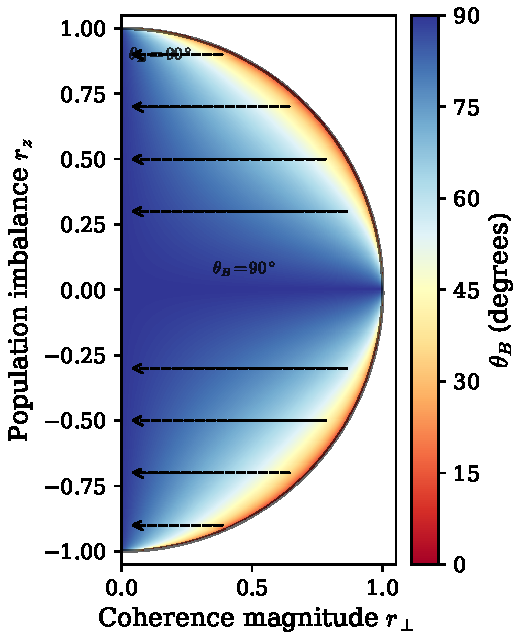
\includegraphics[width=0.7\textwidth]{fig5_bures_angle.pdf}
\caption{\textbf{Bures separation angle across the Bloch disk.}  The principal angle $\theta_B$ between the classical tangent subspace $T_\rho^{\mathrm{diag}}$ and the quantum tangent subspace $T_\rho^{\mathrm{off}}$, plotted on the $(r_\perp, r_z)$ cross-section of the Bloch ball interior $(|\mathbf{r}| < 1)$.  The angle equals $\pi/2$ (perfect orthogonality) on both axes ($r_\perp = 0$ and $r_z = 0$) and decreases toward the pure-state boundary where both coherence and population imbalance are large.  Dashed horizontal arrows show dephasing trajectories at fixed $r_z$, along which $\theta_B$ increases monotonically toward~$\pi/2$.}
\label{fig:bures-angle}
\end{figure}

%% ============================================================
\section{Thermodynamic Cost of Dimensional Collapse}
\label{sec:thermodynamics}
The dimensional collapse from $d^2 - 1$ to $d - 1$ is not free.  Destroying quantum coherences---collapsing the information-geometric dimensions that distinguish quantum from classical state spaces---has a thermodynamic cost.  We now derive this cost using the non-equilibrium free energy decomposition \cite{lostaglio2015description,korzekwa2016extraction}.

\begin{proposition}[Free energy of coherence]
\label{prop:free-energy-coherence}
Let $\rho$ be a quantum state with system Hamiltonian $H$, and let $\Lambda_{\mathrm{dec}}$ be the complete dephasing channel \emph{(Definition~\ref{def:decoherence-channel})}.  The free energy change under dephasing is
\begin{equation}
\label{eq:free-energy-general}
F(\rho) - F(\Lambda_{\mathrm{dec}}[\rho]) = \mathrm{Tr}\bigl[(\rho - \Lambda_{\mathrm{dec}}[\rho])\, H\bigr] + k_B T\, C_r(\rho),
\end{equation}
where $F(\rho) = \mathrm{Tr}[\rho H] - k_B T\, S(\rho)$ is the non-equilibrium free energy, $S(\rho) = -\mathrm{Tr}[\rho \ln \rho]$ is the von Neumann entropy, and $C_r(\rho) = S(\Lambda_{\mathrm{dec}}[\rho]) - S(\rho) \geq 0$ is the relative entropy of coherence \cite{streltsov2017colloquium}.
\end{proposition}

\begin{proof}
By definition of the non-equilibrium free energy:
\[
F(\rho) - F(\Lambda_{\mathrm{dec}}[\rho]) = \mathrm{Tr}[\rho H] - k_B T\, S(\rho) - \mathrm{Tr}[\Lambda_{\mathrm{dec}}[\rho]\, H] + k_B T\, S(\Lambda_{\mathrm{dec}}[\rho]).
\]
Rearranging:
\[
= \mathrm{Tr}\bigl[(\rho - \Lambda_{\mathrm{dec}}[\rho])\, H\bigr] + k_B T \bigl[S(\Lambda_{\mathrm{dec}}[\rho]) - S(\rho)\bigr].
\]
The entropy difference $S(\Lambda_{\mathrm{dec}}[\rho]) - S(\rho) \geq 0$ because $\Lambda_{\mathrm{dec}}$ is unital, so the eigenvalues of $\rho$ majorize those of $\Lambda_{\mathrm{dec}}[\rho]$ and von Neumann entropy is Schur-concave.  The identification $C_r(\rho) = S(\Lambda_{\mathrm{dec}}[\rho]) - S(\rho) = S(\rho \,\|\, \Lambda_{\mathrm{dec}}[\rho])$ is standard \cite{streltsov2017colloquium}: since $\Lambda_{\mathrm{dec}}[\rho] = \sum_k p_k |k\rangle\langle k|$ is diagonal in the pointer basis, $\mathrm{Tr}[\rho \ln \Lambda_{\mathrm{dec}}[\rho]] = \sum_k p_k \ln p_k = -S(\Lambda_{\mathrm{dec}}[\rho])$.
\end{proof}

\begin{corollary}[Dephasing-diagonal Hamiltonian]
\label{cor:diagonal-hamiltonian}
When $H$ is diagonal in the dephasing basis (i.e., every dephasing projector $|k\rangle\langle k|$ commutes with $H$), the energy term vanishes and
\begin{equation}
\label{eq:free-energy-diagonal-H}
F(\rho) - F(\Lambda_{\mathrm{dec}}[\rho]) = k_B T\, C_r(\rho) \;\geq\; 0.
\end{equation}
\end{corollary}

\begin{proof}
When $H$ is diagonal in the pointer basis, $H = \sum_k E_k |k\rangle\langle k|$.  Then $\mathrm{Tr}[\rho H] = \sum_k E_k \langle k|\rho|k\rangle = \sum_k E_k\, p_k = \mathrm{Tr}[\Lambda_{\mathrm{dec}}[\rho]\, H]$, so the energy term in~\eqref{eq:free-energy-general} vanishes.  Non-negativity follows from $C_r(\rho) \geq 0$ by unitality of $\Lambda_{\mathrm{dec}}$.
\end{proof}

\begin{remark}[Geometric correspondence]
\label{rem:geometric-correspondence}
The classical free energy $F(\Lambda_{\mathrm{dec}}[\rho])$ is associated with the $d - 1$ surviving population dimensions (Theorem~\ref{thm:dim-collapse}).  The coherent free energy $k_B T \cdot C_r(\rho)$ is associated with the $d^2 - d$ collapsing off-diagonal directions.  When $H$ is diagonal in the dephasing basis, the free energy decomposes cleanly along the orthogonal subspaces of Theorem~\ref{thm:orthogonal-decomposition}: the classical component on $T_\rho^{\mathrm{diag}}$ and the coherent component on $T_\rho^{\mathrm{off}}$.
\end{remark}

Proposition~\ref{prop:free-energy-coherence} states that decoherence irreversibly destroys non-equilibrium free energy proportional to the coherence content of the state.  A state with no coherence ($C_r = 0$) is already classical---no free energy is stored in coherences.  A maximally coherent state (e.g., $|\psi\rangle = d^{-1/2} \sum_k |k\rangle$) stores the maximum coherent free energy: $C_r = \ln d$.  The dimensions annihilated in Theorem~\ref{thm:dim-collapse}---the $d^2 - d$ off-diagonal directions whose Fisher information vanishes under $\Lambda_{\mathrm{dec}}$---are precisely those whose destruction generates entropy and reduces free energy.

We note that the relationship between coherence and extractable work is operationally subtle: the free energy $k_B T \cdot C_r$ is not in general directly extractable as work without additional resources such as a coherent reference frame \cite{lostaglio2015description,korzekwa2016extraction}.  The identity~\eqref{eq:free-energy-general} is exact as a free energy accounting; its operational interpretation requires care.

\begin{proposition}[Classical limit]
\label{prop:classical-limit}
When $\rho$ is already diagonal in the pointer basis $(\rho = \mathrm{diag}(p))$, $C_r(\rho) = 0$ and $\Delta F = 0$---no free energy is stored in coherences and none is destroyed by dephasing.
\end{proposition}

\begin{proof}
When $\rho$ is diagonal, $\Lambda_{\mathrm{dec}}[\rho] = \rho$, so $C_r(\rho) = S(\rho \,\|\, \rho) = 0$ and $F(\rho) = F(\Lambda_{\mathrm{dec}}[\rho])$.
\end{proof}

\begin{remark}[Classical coarse-graining]
\label{rem:classical-coarse-graining}
Classical coarse-graining (projecting a fine-grained probability distribution onto coarser bins) and quantum dephasing are complementary entropy-increasing processes: both map to lower-dimensional descriptions, but they operate in different directions (populations vs.\ coherences) and are not nested.  The classical Landauer bound \cite{landauer1961irreversibility,bennett1982thermodynamics} applies to the former; Proposition~\ref{prop:free-energy-coherence} applies to the latter.
\end{remark}

\begin{remark}[Cost scaling with system size]
\label{rem:cost-scaling}
For a $d$-dimensional system in a maximally coherent pure state with $H$ diagonal in the dephasing basis, the free energy destroyed by decoherence is $\Delta F = k_B T \ln d$.  Since the dimensional collapse eliminates $d^2 - d$ information-geometric dimensions (Theorem~\ref{thm:dim-collapse}), the cost per collapsed dimension is approximately
\begin{equation}
\label{eq:cost-per-dim}
\frac{\Delta F}{d^2 - d} \;=\; \frac{k_B T \ln d}{d^2 - d} \;\approx\; \frac{k_B T \ln d}{d^2},
\end{equation}
which decreases with system size.  Classicality becomes thermodynamically cheap per degree of freedom for large systems.  This is consistent with the observation that macroscopic decoherence is both fast---Zurek estimates decoherence times of order $10^{-31}$\,s for a dust grain in a thermal photon bath \cite{zurek2003decoherence}---and energetically favorable: the per-dimension cost of erasing quantum coherence vanishes in the macroscopic limit, so the environment pays a negligible price per degree of freedom to enforce classicality.  The total cost $k_B T \ln d$ grows only logarithmically with Hilbert space dimension, while the number of destroyed dimensions grows quadratically.  This asymmetry explains why the quantum-to-classical transition is not merely possible but \emph{generic}: the thermodynamic barrier to classicality is sublinear in the size of the quantum state space that must be collapsed.
\end{remark}

%% ============================================================
\section{Worked Examples}
\label{sec:examples}

We now apply the dimensional collapse framework to concrete physical systems, proceeding from the simplest (a single qubit) through multi-qubit registers and continuous environment models to thermodynamic cost calculations.  These examples serve two purposes: they verify the abstract results of Sections~\ref{sec:decoherence}--\ref{sec:thermodynamics} in exactly solvable cases, and they build physical intuition for how dimensional collapse unfolds in practice.

\subsection{Qubit dephasing}
\label{sec:qubit-dephasing}

Consider a single qubit ($d = 2$) with Bloch vector $\mathbf{r} = (\sin\theta\cos\phi,\; \sin\theta\sin\phi,\; \cos\theta)$, parameterized by the polar angle $\theta \in [0,\pi]$ and azimuthal angle $\phi \in [0,2\pi)$.  The full quantum state manifold $\mathcal{M}_Q$ is the Bloch ball: a three-dimensional solid sphere ($d^2 - 1 = 3$), with pure states on the surface ($|\mathbf{r}| = 1$) and the maximally mixed state at the origin.

Under partial dephasing with parameter $\gamma \in [0, 1/2]$, the Bloch vector transforms as
\begin{equation}
\label{eq:bloch-dephasing}
\mathbf{r} \;\mapsto\; \bigl((1-2\gamma)\sin\theta\cos\phi,\; (1-2\gamma)\sin\theta\sin\phi,\; \cos\theta\bigr).
\end{equation}
The $z$-component (population difference) is preserved, while the $x$- and $y$-components (coherences) are multiplied by the shrinking factor $(1-2\gamma)$.  Geometrically, the Bloch sphere contracts to an oblate ellipsoid with equatorial radius $(1-2\gamma)$ and polar radius~$1$.  At complete dephasing ($\gamma = 1/2$), the ellipsoid collapses to the line segment $[-1,1]$ along the $z$-axis: a one-dimensional manifold ($d - 1 = 1$), exactly as predicted by Theorem~\ref{thm:dim-collapse}.

The quantum Fisher information matrix for the two-parameter family $(\theta, \phi)$ can be computed directly from the SLD equation~\eqref{eq:sld}.  For the dephased state with Bloch vector~\eqref{eq:bloch-dephasing}, one obtains
\begin{equation}
\label{eq:qfim-qubit}
F_Q(\gamma) = \mathrm{diag}\!\left(1,\; (1-2\gamma)^2 \sin^2\theta\right).
\end{equation}
The $\theta$-direction (population parameter) retains unit Fisher information regardless of dephasing.  The $\phi$-direction (phase parameter) loses Fisher information quadratically in $(1-2\gamma)$, consistent with the Bloch-representation analysis of \cite{lu2013fisher}, and the factor $\sin^2\theta$ reflects the fact that states near the poles ($\theta \approx 0, \pi$) have little phase information to lose.

For equatorial states ($\theta = \pi/2$), which carry maximal coherence and therefore suffer the most dramatic collapse, the effective quantum dimensionality~\eqref{eq:deff} evaluates to
\begin{equation}
\label{eq:deff-qubit}
D_{\mathrm{eff}}^Q(\gamma) = \frac{\bigl(1 + (1-2\gamma)^2\bigr)^2}{1 + (1-2\gamma)^4}.
\end{equation}
This decreases monotonically from $D_{\mathrm{eff}}^Q(0) = 2$ (full quantum: both $\theta$ and $\phi$ are equally estimable) to $D_{\mathrm{eff}}^Q(1/2) = 1$ (classical: only the population parameter $\theta$ survives).  Figure~\ref{fig:bloch} illustrates both the geometric collapse and the $D_{\mathrm{eff}}^Q$ trajectory.

\begin{figure}[H]
\centering
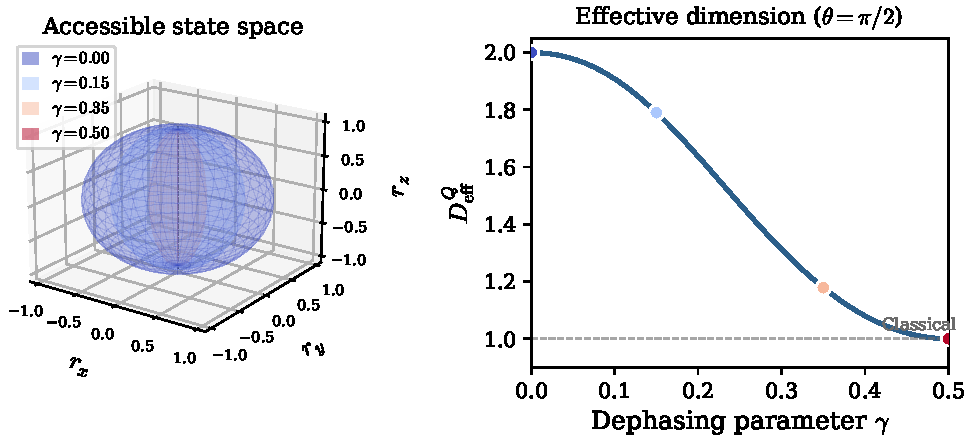
\includegraphics[width=\textwidth]{fig1_bloch_collapse.pdf}
\caption{\textbf{Dimensional collapse of a qubit under dephasing.} Left: the Bloch sphere (the space of qubit states) shrinks under the dephasing channel. The $x$- and $y$-components of the Bloch vector are multiplied by $(1-2\gamma)$ while the $z$-component is preserved, producing an oblate ellipsoid that collapses to the $z$-axis at $\gamma = 1/2$. Right: the effective quantum dimensionality $D_{\mathrm{eff}}^Q$ decreases from 2 (full quantum, both parameters estimable) to 1 (classical, only the population parameter survives). The four marked points correspond to the dephasing levels shown on the left.}
\label{fig:bloch}
\end{figure}

This example makes the abstract content of Theorem~\ref{thm:dim-collapse} visually concrete: the quantum-to-classical transition is literally the collapse of a sphere to a line.  The off-diagonal directions of $\mathcal{M}_Q$---the equatorial plane of the Bloch ball---are exactly the dimensions annihilated by dephasing.  The surviving $z$-axis is the classical probability simplex $\Delta_1$ (a line segment from $|0\rangle\langle 0|$ to $|1\rangle\langle 1|$), equipped with the Fisher--Rao metric inherited from the Bures geometry (Theorem~\ref{thm:metric-restriction}).

\subsection{\texorpdfstring{$N$}{N}-qubit register}
\label{sec:n-qubit}

The qubit example generalizes immediately to $N$-qubit registers under collective dephasing in the computational basis.  For $N$ qubits, the Hilbert space dimension is $d = 2^N$, and Theorem~\ref{thm:dim-collapse} gives:
\begin{itemize}
\item Quantum state space dimension: $d^2 - 1 = 4^N - 1$,
\item Classical state space dimension (after dephasing): $d - 1 = 2^N - 1$,
\item Collapse ratio: $(d - 1)/(d^2 - 1) = 1/(d + 1) = 1/(2^N + 1)$.
\end{itemize}

\begin{table}[H]
\centering
\begin{tabular}{rrrrl}
\hline
$N$ & $d$ & Quantum dims & Classical dims & Fraction surviving \\
\hline
1  & 2     & 3            & 1              & 33.3\% \\
2  & 4     & 15           & 3              & 20.0\% \\
5  & 32    & 1\,023       & 31             & 3.0\% \\
10 & 1\,024 & $\sim\! 10^6$ & 1\,023       & 0.098\% \\
20 & $\sim\! 10^6$ & $\sim\! 10^{12}$ & $\sim\! 10^6$ & $\sim\! 10^{-4}\%$ \\
\hline
\end{tabular}
\caption{Dimensional collapse for $N$-qubit registers.}
\label{tab:n-qubit}
\end{table}

The exponential scaling of the collapse ratio is the quantitative content of the statement that ``almost all information-geometric dimensions are quantum.''  By $N = 10$ qubits---a modest system by any experimental standard---less than $0.1\%$ of the information-geometric degrees of freedom survive the transition to classicality (Figure~\ref{fig:fraction}).  For a system of $N = 20$ qubits, only about one part in a million of the state space carries over to the classical description.  The quantum-to-classical transition is not a gentle reduction; it is a catastrophic dimensional collapse that discards nearly everything.

\begin{figure}[H]
\centering
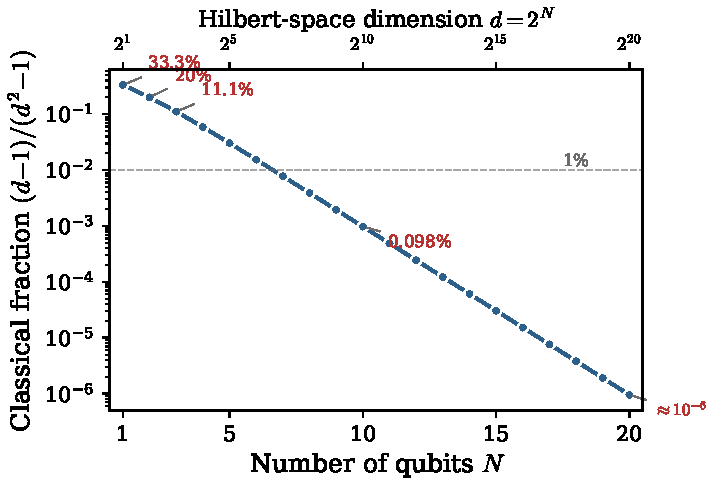
\includegraphics[width=0.7\textwidth]{fig2_classical_fraction.pdf}
\caption{\textbf{Classical dimensionality ratio.} The ratio $(d-1)/(d^2-1) = 1/(d+1)$ of classically surviving dimensions to total quantum dimensions, plotted against the number of qubits $N$ ($d = 2^N$). By $N = 10$ qubits, less than $0.1\%$ of the information-geometric degrees of freedom survive the quantum-to-classical transition.}
\label{fig:fraction}
\end{figure}

\subsection{Spin-boson model}
\label{sec:spin-boson}

The previous examples used discrete dephasing steps.  We now consider a physically motivated continuous-time model: a qubit coupled to a bosonic thermal bath, described by the spin-boson model of Leggett et al.\ \cite{leggett1987dynamics}.  The environment is characterized by an Ohmic spectral density
\begin{equation}
\label{eq:spectral-density}
J(\omega) = \eta\,\omega\, e^{-\omega/\omega_c},
\end{equation}
where $\eta$ is the dimensionless coupling strength and $\omega_c$ is a high-frequency cutoff.

In the high-temperature Markovian regime ($k_BT \gg \hbar\omega_c$), the off-diagonal element of the reduced density matrix decays exponentially:
\begin{equation}
\label{eq:spin-boson-decay}
\rho_{01}(t) = \rho_{01}(0)\, e^{-\Gamma(t)}, \qquad \Gamma(t) = \eta k_BT\, t.
\end{equation}
The decoherence function $\Gamma(t)$ grows linearly in time, with a rate set by the product of coupling strength and temperature.

Mapping this to the qubit dephasing analysis of Section~\ref{sec:qubit-dephasing} (with $(1 - 2\gamma) \to e^{-\Gamma(t)}$), the quantum Fisher information for the phase parameter at $\theta = \pi/2$ is
\begin{equation}
\label{eq:qfi-spinboson}
F_\phi(t) = e^{-2\Gamma(t)} = e^{-2\eta k_BT\, t},
\end{equation}
and the effective quantum dimensionality follows the trajectory
\begin{equation}
\label{eq:deff-spinboson}
D_{\mathrm{eff}}^Q(t) = \frac{\bigl(1 + e^{-2\Gamma(t)}\bigr)^2}{1 + e^{-4\Gamma(t)}}.
\end{equation}
This defines a characteristic timescale for dimensional collapse (in units where $\hbar = 1$):
\begin{equation}
\label{eq:tau-dec}
\tau_{\mathrm{dec}} \sim \frac{1}{2\eta k_BT}.
\end{equation}
After one decoherence time $\tau_{\mathrm{dec}}$, the effective quantum dimensionality has dropped roughly halfway from its quantum value of~$2$ to the classical value of~$1$.  Figure~\ref{fig:trajectories} shows $D_{\mathrm{eff}}^Q(t)$ for several values of $\eta k_BT$.

\begin{figure}[H]
\centering
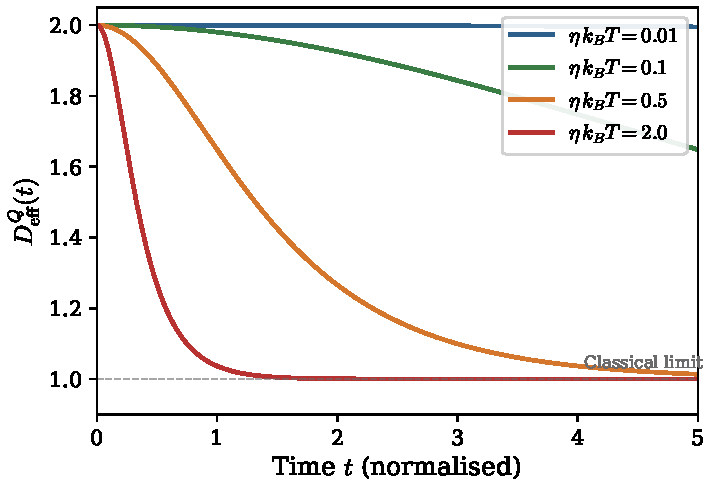
\includegraphics[width=0.7\textwidth]{fig3_deff_trajectories.pdf}
\caption{\textbf{Dimensional collapse under spin-boson decoherence.} The effective quantum dimensionality $D_{\mathrm{eff}}^Q(t)$ for a qubit coupled to an Ohmic bosonic bath at high temperature, for four coupling strengths $\eta k_BT$. Weak coupling (0.01) preserves near-quantum dimensionality over the displayed time window; strong coupling (2.0) drives collapse to the classical value $D_{\mathrm{eff}}^Q = 1$ within $t \sim 1$. All curves share the same functional form but with different characteristic timescales.}
\label{fig:trajectories}
\end{figure}

An important subtlety concerns the short-time behavior.  The Markovian approximation $\Gamma(t) = \eta k_BT\, t$ is valid only for $t \gg 1/\omega_c$.  At very short times ($t \ll 1/\omega_c$), the exact decoherence function is quadratic: $\Gamma(t) \sim (\eta k_BT\, \omega_c)\, t^2$, reflecting the quantum Zeno regime in which frequent environmental interactions initially suppress decoherence \cite{leggett1987dynamics}.  The initial decay of $D_{\mathrm{eff}}^Q$ is therefore quadratic, not exponential---a potentially testable prediction that distinguishes the dimensional collapse framework from phenomenological models that assume exponential decay from $t = 0$.  The crossover from Zeno (quadratic) to Markovian (exponential) dimensional collapse occurs at $t \sim 1/\omega_c$, and the full trajectory depends on the spectral structure of the bath, not merely on a single decoherence rate.

\subsection{Thermodynamic cost in action}
\label{sec:thermo-example}

We now illustrate Proposition~\ref{prop:free-energy-coherence} for a qubit initially prepared in the maximally coherent state $|{+}\rangle = (|0\rangle + |1\rangle)/\sqrt{2}$, with $H$ diagonal in the dephasing basis so that Corollary~\ref{cor:diagonal-hamiltonian} applies.  Under partial dephasing with parameter $\gamma$, the state becomes
\begin{equation}
\label{eq:dephased-plus}
\rho(\gamma) = \begin{pmatrix} 1/2 & (1-2\gamma)/2 \\ (1-2\gamma)/2 & 1/2 \end{pmatrix},
\end{equation}
which has eigenvalues $(1 \pm (1-2\gamma))/2$.  The von Neumann entropy is therefore
\begin{equation}
\label{eq:entropy-dephased}
S(\rho(\gamma)) = H_2\!\left(\frac{1 + (1-2\gamma)}{2}\right),
\end{equation}
where $H_2(p) = -p\ln p - (1-p)\ln(1-p)$ is the binary entropy function.

Since the diagonal elements are $(1/2, 1/2)$ for all values of $\gamma$---dephasing preserves populations---the fully decohered state is always the maximally mixed state:
\begin{equation}
\label{eq:decohered-entropy}
S(\Lambda_{\mathrm{dec}}[\rho(\gamma)]) = \ln 2.
\end{equation}

By Corollary~\ref{cor:diagonal-hamiltonian}, the free energy destroyed by the remaining dephasing (from $\gamma$ to $1/2$) is
\begin{equation}
\label{eq:cost-qubit}
\frac{\Delta F}{k_BT} = C_r(\gamma) = \ln 2 - H_2\!\left(\frac{1+(1-2\gamma)}{2}\right).
\end{equation}

The limiting cases are instructive.  At $\gamma = 0$ (pure state $|{+}\rangle$), the entropy vanishes ($S(\rho) = 0$) and the full coherent free energy equals $\Delta F = k_BT \ln 2 \approx 0.693\, k_BT$.  This is the free energy stored in one bit of quantum coherence.  At $\gamma = 1/2$ (complete dephasing), the state is already maximally mixed and $C_r = 0$: no coherent free energy remains, consistent with Proposition~\ref{prop:classical-limit}.  Between these extremes, the coherent free energy decreases monotonically as dephasing progressively destroys coherence and the state approaches classicality.

\begin{figure}[H]
\centering
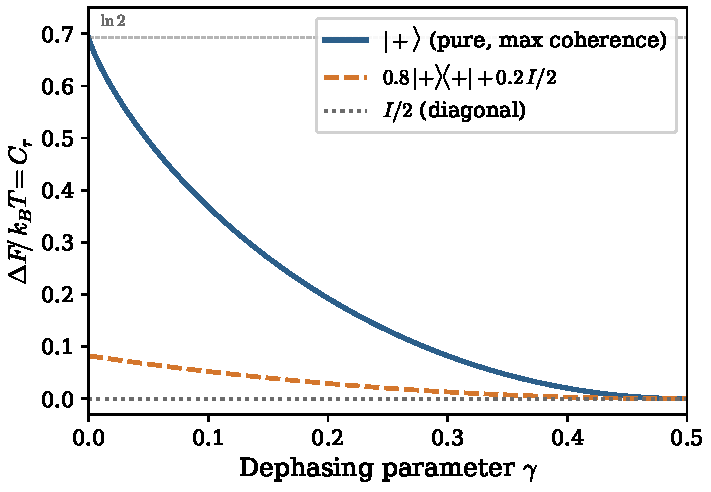
\includegraphics[width=0.7\textwidth]{fig4_quantum_dlb.pdf}
\caption{\textbf{Free energy destroyed by dimensional collapse.} The coherent free energy $\Delta F/k_BT = C_r$ as a function of dephasing parameter $\gamma$ for three initial qubit states. The maximally coherent state $|{+}\rangle$ stores the full coherent free energy $\ln 2$ at $\gamma = 0$; this decreases as dephasing progressively destroys coherence. A partially coherent mixed state starts with reduced coherent free energy. An already-diagonal state (classical) has zero coherent free energy throughout, consistent with Proposition~\ref{prop:classical-limit}.}
\label{fig:dlb}
\end{figure}

The connection between Figures~\ref{fig:bloch} and~\ref{fig:dlb} is the central message of this paper: the geometric collapse (Figure~\ref{fig:bloch}, $D_{\mathrm{eff}}^Q$ falling from~2 to~1) and the destroyed free energy (Figure~\ref{fig:dlb}, $\Delta F$ decreasing from $k_BT \ln 2$ to~0) are two views of the same process.  Each collapsed dimension corresponds to destroyed coherence, and each unit of destroyed coherence corresponds to destroyed free energy.  Proposition~\ref{prop:free-energy-coherence} makes this correspondence quantitative.

%% ============================================================
\section{Pointer States and the Geometry of Einselection}
\label{sec:pointer}

The analysis of Sections~\ref{sec:decoherence}--\ref{sec:examples} assumed a given pointer basis $\{|k\rangle\}$ and studied the resulting collapse.  But where does the pointer basis come from?  This section connects the dimensional collapse framework to Zurek's program of environment-induced superselection (einselection), which provides the physical mechanism selecting the pointer basis, and to quantum Darwinism, which explains why the resulting classical projection appears objective.

\subsection{Basis dependence of the target simplex}
\label{sec:basis-dependence}

The decoherence channel $\Lambda_{\mathrm{dec}}$ (Definition~\ref{def:decoherence-channel}) depends on the choice of pointer basis $\{|k\rangle\}$.  Different orthonormal bases define different decoherence channels, and each such channel projects the quantum state manifold $\mathcal{M}_Q$ onto a different embedding of $\Delta_{d-1}$ within $\mathcal{M}_Q$.

All target simplices are isomorphic as topological spaces: each is a $(d-1)$-dimensional simplex, with the same combinatorial structure of vertices, edges, and faces.  However, the simplices carry different \emph{Fisher--Rao metrics} induced by the Bures metric of the ambient quantum manifold.  For a given pointer basis $\{|k\rangle\}$, the embedding
\begin{equation}
\label{eq:simplex-embedding}
\iota_{\{|k\rangle\}}: \Delta_{d-1} \hookrightarrow \mathcal{M}_Q, \qquad p \mapsto \sum_k p_k |k\rangle\langle k|,
\end{equation}
equips the simplex with the metric inherited from $\mathcal{M}_Q$ along this particular submanifold.  By Theorem~\ref{thm:metric-restriction}, this inherited metric is the Fisher--Rao metric---but the \emph{location} of the simplex within $\mathcal{M}_Q$, and hence the geometric relationship between classical states and the surrounding quantum state space, depends on the choice of basis.

The choice of pointer basis therefore determines \emph{which} classical distinctions are preserved by decoherence.  In the qubit example of Section~\ref{sec:qubit-dephasing}, dephasing in the $z$-basis collapses the Bloch sphere onto the $z$-axis, preserving the distinction between $|0\rangle$ and $|1\rangle$ (spin up vs.\ spin down along $z$).  Dephasing in the $x$-basis would instead collapse onto the $x$-axis, preserving the distinction between $|{+}\rangle$ and $|{-}\rangle$.  The two collapses annihilate the same \emph{number} of dimensions ($d^2 - d = 2$ in both cases), but they annihilate \emph{different} dimensions.  The dimensional collapse is basis-dependent in its content, even as it is basis-independent in its magnitude.

\subsection{Einselection as geometry selection}
\label{sec:einselection}

Zurek's einselection (environment-induced superselection) \cite{zurek2003decoherence,zurek2025decoherence} provides the physical mechanism that resolves the basis ambiguity identified in Section~\ref{sec:basis-dependence}.  When a system $S$ interacts with an environment $E$ through a Hamiltonian
\begin{equation}
\label{eq:interaction-hamiltonian}
H_{SE} = \sum_k |s_k\rangle\langle s_k| \otimes B_k
\end{equation}
(written in its Schmidt decomposition, where $\{|s_k\rangle\}$ are orthonormal system states and $B_k$ are environment operators), the pointer states $\{|s_k\rangle\}$ are exactly the states that commute with $H_{SE}$ and hence survive the interaction without being perturbed.  Superpositions of pointer states, by contrast, become entangled with the environment and decohere into mixtures.

In the language of the dimensional collapse framework: einselection determines \emph{which} $(d-1)$-dimensional submanifold $\mathcal{M}_Q$ collapses onto.  The pointer basis is not selected by any optimization of $D_{\mathrm{eff}}^Q$---the collapse magnitude $d^2 - 1 \to d - 1$ is the same for all choices of basis.  Rather, the pointer basis is determined by the physics of the system--environment interaction: the eigenstates of $H_{SE}$ in the system factor.  What $D_{\mathrm{eff}}^Q$ measures is the \emph{outcome}: it quantifies how many operationally distinguishable degrees of freedom survive the collapse, and Corollary~\ref{cor:deff-collapse} guarantees this number cannot exceed $d - 1$ regardless of which basis is selected.

The geometric picture is therefore a two-stage process:
\begin{enumerate}
\item \emph{Einselection} (physics) selects the pointer basis $\{|s_k\rangle\}$, thereby fixing the target simplex $\iota_{\{|s_k\rangle\}}(\Delta_{d-1}) \subset \mathcal{M}_Q$.
\item \emph{Decoherence} (dynamics) drives the state toward this simplex, collapsing $D_{\mathrm{eff}}^Q$ from its quantum value toward the classical bound $d - 1$.
\end{enumerate}
Einselection selects the geometry; decoherence executes the collapse.

\subsection{Quantum Darwinism as redundant projection}
\label{sec:darwinism}

Zurek's quantum Darwinism \cite{zurek2003decoherence,zurek2025decoherence,riedel2010zurek} addresses a further question: why does the classical world appear \emph{objective}---why do different observers agree on the outcome of decoherence?  The answer is that pointer states are not merely preserved; they are \emph{replicated} in the environment.  As the system interacts with many environmental degrees of freedom, information about the pointer state is recorded redundantly in multiple independent environmental fragments.

In the dimensional collapse framework, the environment acquires multiple independent copies of the $(d-1)$-dimensional classical projection.  Each environmental fragment---a subset of the bath degrees of freedom that has interacted with the system---contains a copy of the same simplex $\Delta_{d-1}$ with the same Fisher--Rao metric.  This is what makes the classical world ``objective'' in Zurek's sense: all observers agree because they observe the same dimensional collapse to the same target simplex.  Zurek's ``consensus'' is the statement that all environmental projections share the same pointer basis, and hence the same target geometry.

The redundancy quantified by Riedel and Zurek \cite{riedel2010zurek}---approximately $10^7$ independent copies of a dust grain's position recorded in scattered photons within a single microsecond---means that the classical projection is massively overdetermined.  From the information-geometric perspective, this redundancy is the mechanism by which a single $(d-1)$-dimensional projection becomes stable against perturbation: even if some environmental records are lost, the consensus survives.  The classical world is robust precisely because it is a low-dimensional projection that has been copied many times.

This redundancy also explains the apparent irreversibility of the quantum-to-classical transition.  In principle, decoherence is unitary at the level of system-plus-environment: no information is destroyed, merely redistributed.  But reversing the collapse would require recovering coherent information from $\sim\!10^7$ environmental fragments and restoring their phase relationships---a task that would require reversing the entropy increase, at a work cost of at least $k_B T \cdot C_r$ per degree of freedom (Proposition~\ref{prop:free-energy-coherence}).  The thermodynamic cost of ``un-collapsing'' a macroscopic dimensional collapse, recoherence of $\sim\!10^7$ scattered records, vastly exceeds any realistic energy budget.  The classical projection, once established and redundantly copied, is for all practical purposes permanent.

%% ============================================================
\section{Discussion}
\label{sec:discussion}

\subsection{What this resolves}
\label{sec:resolves}

The quantum-to-classical transition has a precise geometric characterization: it is a dimensional collapse from $d^2 - 1$ to $d - 1$ in the quantum Fisher information manifold. The collapsed dimensions are specifically the quantum coherences---the $d^2 - d$ off-diagonal parameters that encode phase relationships between pointer states. The surviving dimensions are the $d - 1$ classical populations. The free energy destroyed equals $k_B T$ times the coherence content of the state when the Hamiltonian is diagonal in the dephasing basis (Proposition~\ref{prop:free-energy-coherence}).

The Bures separation angle (Theorem~\ref{thm:bures-angle}) adds a dynamical dimension to this picture: the geometric separation between classical and quantum degrees of freedom is not fixed but state-dependent.  The classical--quantum tangent split is oblique exactly when the state simultaneously carries nonzero coherence and nonzero population imbalance; dephasing monotonically restores orthogonality.  This means the clean geometric distinction between classical and quantum information---the orthogonal decomposition of Theorem~\ref{thm:orthogonal-decomposition}---is not a pre-existing feature of the state space but an \emph{outcome} of the decoherence process itself.

This characterization is substrate-independent: it applies to any quantum system, any pointer basis, and any decoherence mechanism that can be described as a CPTP map satisfying the conditions of Theorem~\ref{thm:dim-collapse}. The ratio $(d-1)/(d^2-1) = 1/(d+1)$ of surviving classical dimensions to total quantum dimensions is a universal feature of the dimensional structure of decoherence. It depends only on the Hilbert space dimension $d$, not on the details of the system--environment interaction, the spectral density of the bath, or the coupling strength. These physical parameters determine the \emph{rate} of collapse (as illustrated by the spin-boson example in Section~\ref{sec:spin-boson}), but the \emph{magnitude}---how many dimensions are ultimately lost---is fixed by the algebraic structure of quantum state space itself. For a 10-qubit system ($d = 1024$), less than $0.1\%$ of the information-geometric degrees of freedom survive the quantum-to-classical transition.

\subsection{What this does not resolve}
\label{sec:not-resolves}

Three aspects of the measurement problem lie outside the scope of this framework.

\emph{The Born rule.} Our framework assumes the standard quantum probability rule throughout. The quantum Fisher information matrix is defined using the Born-rule probabilities for measurement outcomes (Definition~\ref{def:qfim}), and the free energy decomposition (Proposition~\ref{prop:free-energy-coherence}) is derived from the von Neumann entropy, which presupposes the Born rule in its operational interpretation. A derivation of the Born rule from more primitive principles---as attempted by Zurek \cite{zurek2003decoherence} via envariance and by others through decision-theoretic arguments---would strengthen the foundations of this framework but lies outside our scope.

\emph{The specific outcome.} Given a quantum state in superposition, why does a particular measurement yield this result rather than that one? Our framework characterizes the space of possible classical outcomes---the simplex $\Delta_{d-1}$---and the cost of reaching it, but does not explain the selection of a particular point on the simplex. The dimensional collapse tells us \emph{where} classicality lives (on a $(d-1)$-dimensional submanifold) and \emph{what it costs} ($k_BT \cdot C_r(\rho)$ in destroyed free energy), but not \emph{which} classical outcome obtains. This remains the deepest open question in quantum foundations, and no interpretation of quantum mechanics---from Copenhagen to many-worlds---has produced a consensus resolution.

\emph{The timing of commitment.} At what point does a quantum system irrevocably commit to a classical outcome? The dimensional collapse described in this paper is continuous: $D_{\mathrm{eff}}^Q$ is parameterized by the dephasing strength $\gamma$ (or equivalently, by time $t$ in a dynamical model such as the spin-boson example) and interpolates smoothly between its quantum and classical values. There is no sharp transition, no critical $\gamma^*$ at which classicality abruptly appears. This is consistent with the decoherence program's view that classicality emerges gradually, but it does not resolve the question of whether there is a ``moment of fact'' in a given measurement---a question that may ultimately require interpretive commitments beyond those made here.

\subsection{Connection to the epiontic interpretation}
\label{sec:epiontic}

Zurek \cite{zurek2025decoherence} argues that the quantum state is simultaneously epistemic (encoding what can be known) and ontic (encoding what exists)---a position he terms ``epiontic.'' The dimensional collapse framework provides a geometric version of this claim.

The quantum state is ontic in the sense that $d^2 - 1$ real parameters are required to specify it: the full quantum manifold $\mathcal{M}_Q$ is physically real, and all $d^2 - 1$ dimensions are needed to predict the statistics of arbitrary measurements. It is epistemic in the sense that after decoherence, only $d - 1$ classical parameters are accessible to any observer: the remaining $d^2 - d$ coherence dimensions have been projected away by environmental entanglement and can no longer be recovered without reversing the entanglement with $\sim\!10^7$ environmental degrees of freedom (Section~\ref{sec:darwinism}).

The transition from ontic to epistemic is not a change of philosophical stance; it is a geometric projection with a quantifiable thermodynamic cost. The quantum state does not cease to exist upon decoherence---unitarity is preserved at the level of system-plus-environment---but the accessible information-geometric structure collapses from $d^2 - 1$ to $d - 1$ dimensions. The ``epiontic'' nature of quantum states, in this reading, is a consequence of the dimensional mismatch between the quantum manifold and its classical shadow: the full state is ontic ($d^2 - 1$ dimensions exist), while the accessible state is epistemic ($d - 1$ dimensions can be known).

\subsection{Connection to dimensional projection theory}
\label{sec:projection-theory}

This work generalizes prior results on measurement as dimensional collapse in classical systems \cite{todd2025falsifiability,todd2025timing}. The Projection Bound of \cite{todd2025timing}---which quantifies the energetic cost of projecting a high-dimensional continuous system to a low-dimensional measurement record---and the quantum free energy decomposition of Proposition~\ref{prop:free-energy-coherence} are complementary bounds: the classical bound applies to coarse-graining of populations, while Proposition~\ref{prop:free-energy-coherence} applies to dephasing of coherences. They are not nested (Remark~\ref{rem:classical-coarse-graining}).

The participation ratio $D_{\mathrm{eff}}^Q$ introduced here (Definition~\ref{def:deff}) is the natural quantum generalization of the effective dimensionality used in neural and biological systems analysis, where the participation ratio of covariance eigenvalues measures the intrinsic dimensionality of dynamics. The quantum version measures the same quantity---intrinsic dimensionality of distinguishable dynamics---but in the richer geometry of quantum state space, where the relevant metric is the Bures metric rather than the Euclidean metric, and the relevant eigenvalues are those of the quantum Fisher information matrix rather than the covariance matrix.

Two directions for future work emerge naturally from this framework. First, quantum error correction is precisely the attempt to resist dimensional collapse: error-correcting codes maintain quantum coherences (high $D_{\mathrm{eff}}^Q$) against the decoherence channel by encoding logical qubits in subspaces that are insensitive to the dominant error operators. The dimensional collapse framework may provide a geometric characterization of the threshold at which error correction fails---the point at which the decoherence channel overwhelms the code's ability to maintain $D_{\mathrm{eff}}^Q$ above the classical bound. Second, the analysis presented here considers complete dephasing channels. Extending to partial decoherence channels, amplitude damping channels, and more general CPTP maps would characterize dimensional collapse to intermediate manifolds between $\mathcal{M}_Q$ and $\Delta_{d-1}$, where the effective dimensionality saturates at a value strictly between $d - 1$ and $d^2 - 1$. Such intermediate collapses may be relevant to quantum thermodynamics and to the semiclassical regime in which quantum and classical degrees of freedom coexist.

\bibliographystyle{unsrt}
\bibliography{references}

\end{document}
